\chapter{Pure dephasing or Does the density matrix really exist?}

There are two ways of describing pure dephasing. One is developed from the system-bath approach (Lindbladian master equation) and the other comes from the stochastic Schrödinger equation. However, the results of the latter deviate fundamentally from the results of the former for the experiment of spin-echo for a single qubit. Here this problem will be described in detail.

\section{Quantum derivation of dephasing}

For the derivation of this phase-destroying process in a quantum way the system-environment interaction Hamiltonian part is chosen as
\[
\mathcal{\hat H}_{qe} = \hat \sigma_z \otimes \hat O_e, 
\]
where $\hat O_e$ is an arbitrary environment operator. From this interaction term a master equation is then developed:
\[
\partial_t \hat \rho_s = \frac{i}{\hbar}[\hat \rho_s, \mathcal{\hat H}_s] + \frac{\gamma_\phi}{2} (\hat \sigma_z \hat \rho_s \hat \sigma_z - \hat \rho_s).
\]
The dynamics of this equation can be seen in \autoref{fig:qdeph}.  At $t \rightarrow \infty$ the state of the system is a totally mixed state:
\[
\hat \rho_s (\infty) = \rbrkt{\begin{matrix}
\rho_{11}(0) & 0 \\
0 & \rho_{22}(0) 
\end{matrix}}.
\]
Following the open system approach this should be understood as the consequence of the entanglement of the qubit with the environment. The same density matrix we will obtain trying to find out in which state
is the qubit $A$ when it's a part of a composite system $A \otimes B$ of two qubits being in a Bell  state $\ket{\Psi^+} = \frac{1}{\sqrt{2}}(\ket{0}_A\otimes\ket{1}_B+\ket{1}_A\otimes\ket{0}_B)$. From the quantum point of view, therefore, the process of dephasing is irreversible.
\begin{figure}
\centering
\begin{subfigure}[t]{0.45\textwidth}
\centering
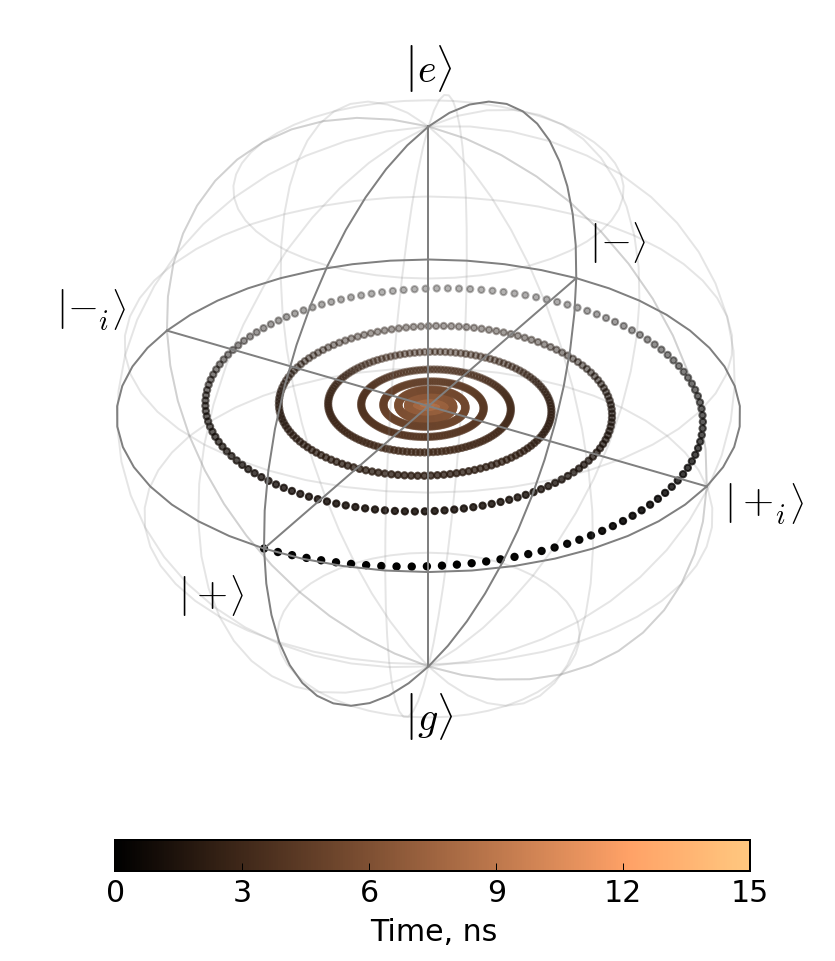
\includegraphics[width=0.9\textwidth]{qdeph_bloch}
\caption{Dephasing on the Bloch sphere.}
\end{subfigure}
\begin{subfigure}[t]{0.45\textwidth}
\centering
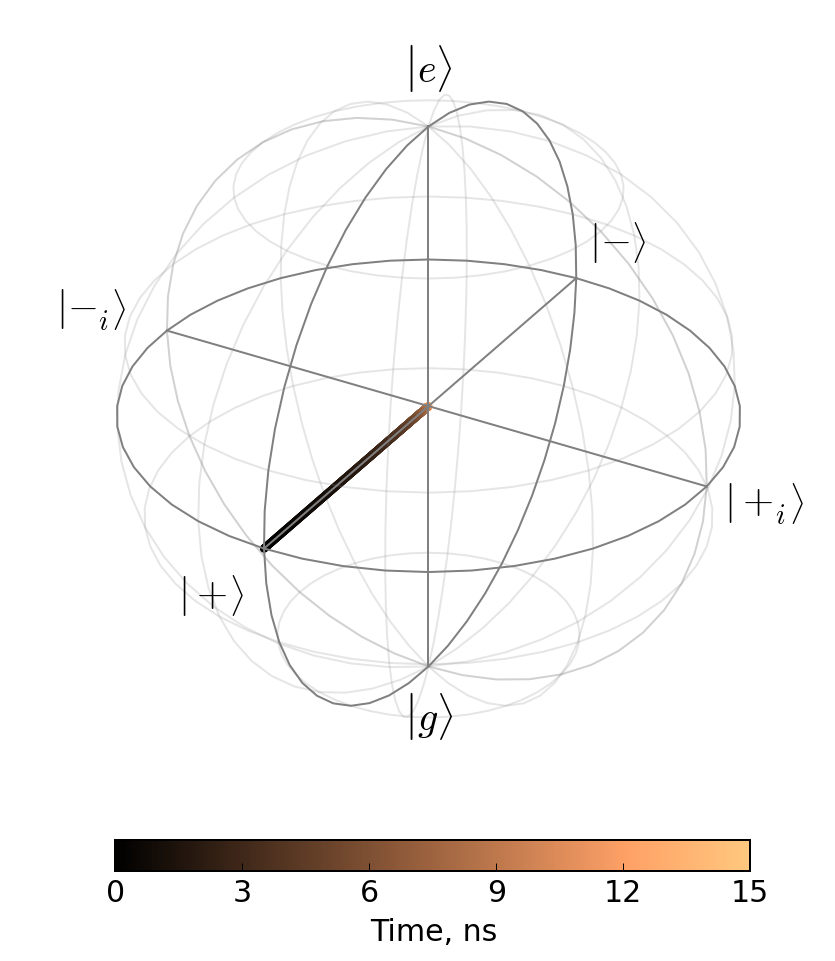
\includegraphics[width=0.9\textwidth]{qdeph_bloch_rf}
\caption{Same within the rotating frame.}
\end{subfigure}

\begin{subfigure}[t]{0.45\textwidth}
\centering
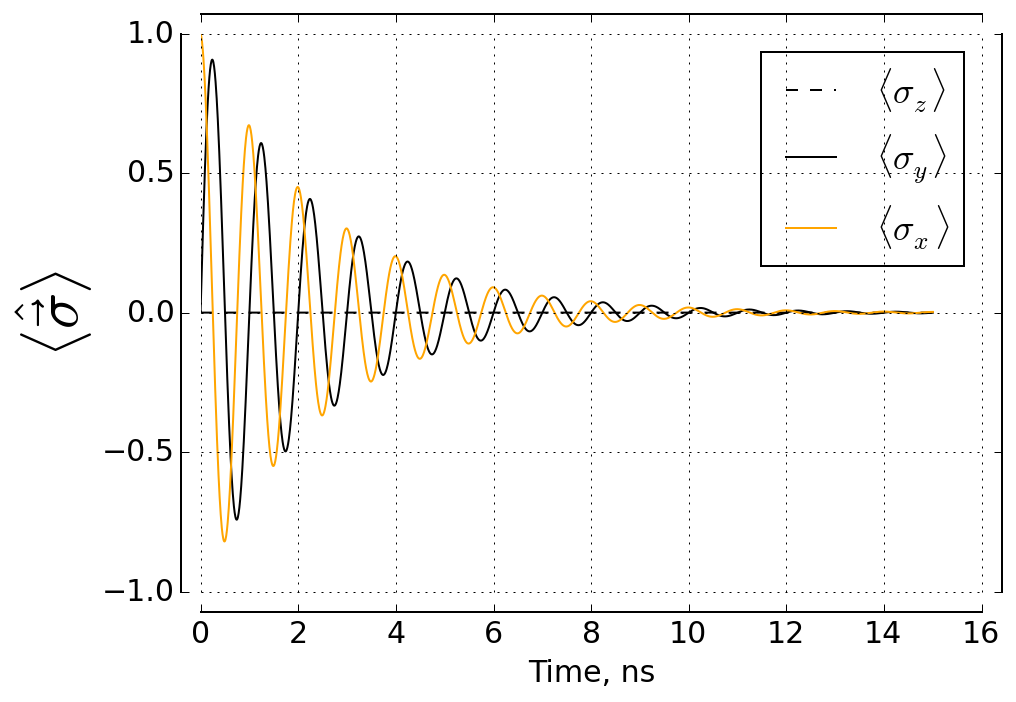
\includegraphics[width=0.9\textwidth]{qdeph_xyz}
\caption{Decay of the $\langle \hat \sigma_{x, y} \rangle$ components.}
\end{subfigure}
\begin{subfigure}[t]{0.45\textwidth}
\centering
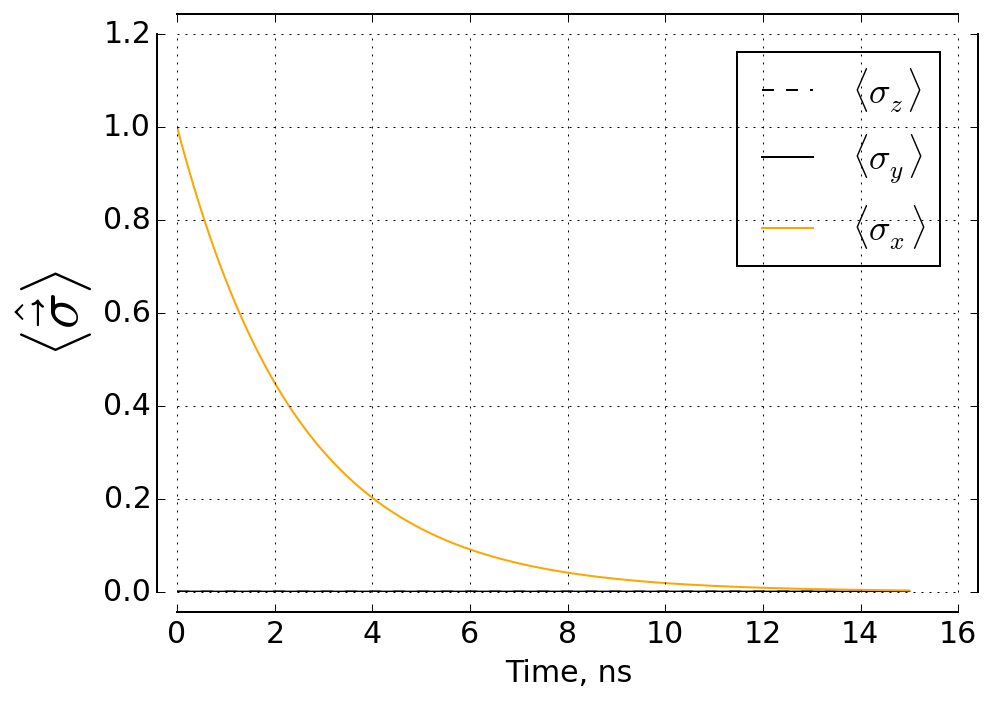
\includegraphics[width=0.9\textwidth]{qdeph_xyz_rf}
\caption{Same within the rotating frame.}
\end{subfigure}
\caption{Dephasing treated quantum-mechanically shows exponential decrease of the coherences of the density matrix.}
\label{fig:qdeph}
\end{figure}

\section{Classical derivation of dephasing}

The classical derivation will be presented below in detail. This method, just as in the case of interaction of an atom with a classical field, just includes an additional time-dependent term in the Hamiltonian, representing fluctuations of the system's parameters. For the pure dephasing this term looks like $f(t) \hat \sigma_z$, where $f(t)$ is the random noise. It is possible to write down the evolution of the density matrix for such stochastic Schrödinger equation. Until specified, the unitary evolution will be discussed, although using density matrix. In the rotating frame:
\[
\hat \rho_s (t) = \hat U^\dag(t, 0)\ \hat\rho\ \hat U(t, 0), 
\]
where 
\[
\hat U(t, 0) = \hat T \exp \left\{-\frac{i}{\hbar} \int_0^t f(\tau)\hat \sigma_z \diff\tau\right\}.
\]
From the fact that $\hat \sigma_z$ is diagonal it can be shown that
\[
\begin{gathered}
\hat \rho_s (t) = \rbrkt{\begin{matrix}
\exp \left\{\frac{i}{\hbar} \int_0^t f(\tau_1) \diff\tau_1\right\} & 0\\
0 & \exp \left\{-\frac{i}{\hbar} \int_0^t f(\tau_1) \diff\tau_1\right\}
\end{matrix}}\cdot\\
\cdot\rbrkt{\begin{matrix}
1/2 - N(0)/2 & \rho(0) \\
\rho^*(0) & 1/2 + N(0)/2 
\end{matrix}}\cdot\\
\cdot\rbrkt{\begin{matrix}
\exp \left\{-\frac{i}{\hbar} \int_0^t f(\tau_2)\diff\tau_2\right\} & 0\\
0 & \exp \left\{+\frac{i}{\hbar} \int_0^t f(\tau_2)\diff\tau_2\right\}
\end{matrix}},
\end{gathered}
\] 
where the integral variables $\tau_1$ and $\tau_2$, coherence $\rho(t)$ and inversion $N(t)$ were introduced. From above it is obvious that
\begin{gather}
N(t) = N(0),\\
\rho(t) = \rho(0)\exp \left\{ \frac{2i}{\hbar}\int_0^t f(\tau)  \diff \tau \right\}. \label{eq:rho_t}
\end{gather}
This equations can be visualized with numerical simulation, taking $f(t)$ be, for instance, normally distributed. The phase will experience random drifts, which lead to random rotations of the Bloch vector on the equator of the sphere, see \autoref{fig:cdeph}~(a), (c).

However, we can now use the other side of the density matrix, the property for which it is also called statistical operator. Let's run the equation \eqref{eq:rho_t} many times and look at the statistically expected state of the observed system over time. The diagonal part will still stay the same, and for coherence we have (presuming Gaussian instantaneous distribution of $f(t)$ and $x(t) = \frac{2}{\hbar}\int_0^t f(\tau)  \diff \tau$):
\begin{gather}
\langle \rho(t) \rangle = \rho(0) \int_{-\infty}^{+\infty} e^{ix}\, \mathbb{N}_{0,\sigma}(x) \diff x = \rho(0) e^{-\sigma^2/2} = \rho(0) e^{-\langle x^2 \rangle/2} \\
= \rho(0)\exp \left\{ -\frac{2}{\hbar^2}\int_0^t\int_0^t \langle f(\tau_1) f(\tau_2) \rangle \diff \tau_1 \diff \tau_2 \right\}.
\end{gather}
Presuming also that $f(t)$ is a wide-sense stationary process $\langle f(\tau_1) f(\tau_2) \rangle = K_f(\tau_2 - \tau_1) = \frac{1}{\sqrt{2\pi}}\int\limits_\mathbb{R} S_f(\omega) e^{i\omega(\tau_2-\tau_1)}\diff\omega$ where $S_f(\omega)$ is the power spectral density of $f(t)$. Taking the time integrals with the exponents, finally we obtain
\begin{equation}
\langle \rho(t) \rangle = \rho(0) \exp  \left\{-\frac{2}{\sqrt{2\pi}\hbar^2} \int\limits_\mathbb{R} W_t^R(\omega) S_f(\omega)\diff \omega \right\},\  W_t^R(\omega)  = \frac{4 \sin^2(\frac{\omega t}{2})}{\omega^2}\label{eq:cdeph}
\end{equation}
It can be shown easily that \eqref{eq:cdeph} is an exponent for either a white noise ($S_f(\omega) = S_f(0) = const$) or for a sufficiently large time $t$ where 
$$\frac{t}{2}\int\limits_\mathbb{R} \diff(\omega t/2) \frac{\sin^2(\frac{\omega t}{2})}{(\omega t/2)^2} \ \bullet $$
acts as $ \frac{t\pi}{2}\delta(\omega)\ \bullet$. In both these cases the pure dephasing rate $\Gamma^*_2$ exists in the usual sense and $\Gamma^*_2 \propto S_f(0)$. In case of, for example, the 1/f noise, the decay curve will behave as $e^{-t^2}$ in the vicinity of $t=0$.

The averaged evolution for the white noise case can be observed in \autoref{fig:cdeph}~(b), (d). It is very similar to what can be seen in \autoref{fig:qdeph}. 1000 trajectories were used for averaging.
In \autoref{fig:cdeph_pink} the simulation of the dynamics under the 1/f noise is shown. For the averaged case ((b), (d)) 2500 trajectories where used. One can see that a plateau is present for the yellow graph near $t=0$, in accordance with theoretical predictions.
\begin{figure}
\begingroup
\captionsetup[subfigure]{width=0.9\textwidth}
\centering
\begin{subfigure}[t]{0.45\textwidth}
\centering
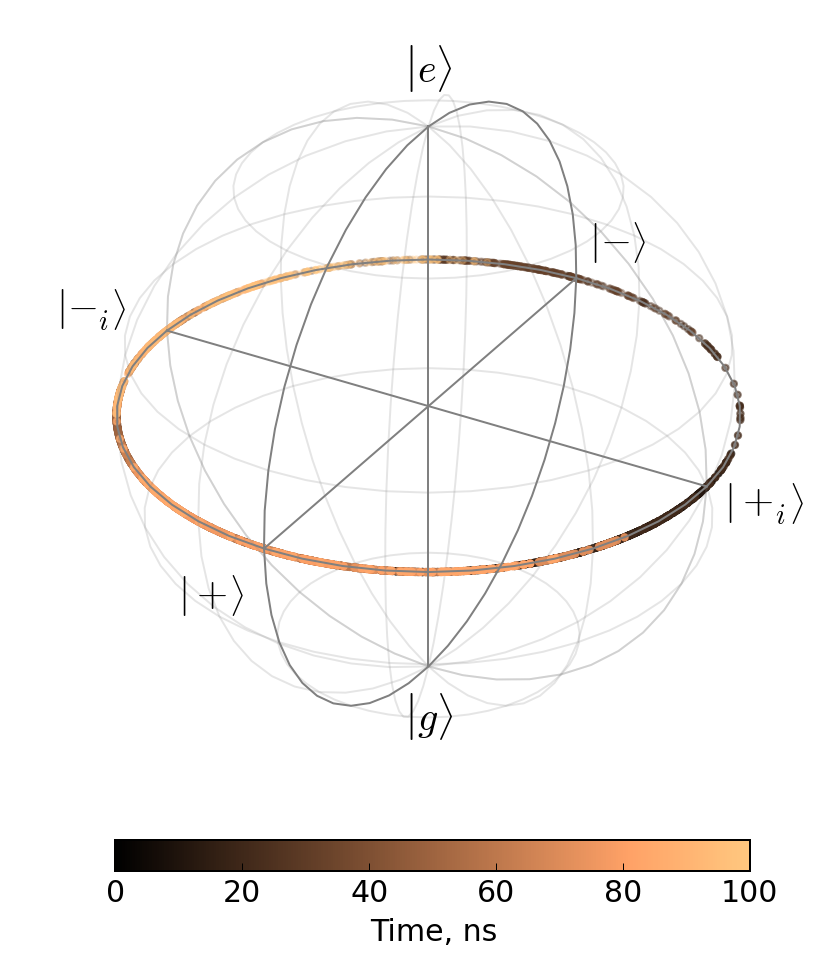
\includegraphics[width=0.9\textwidth]{cdeph_bloch_rf}
\caption{White Gaussian noise affecting the phase in the rotating frame.}
\end{subfigure}
\begin{subfigure}[t]{0.45\textwidth}
\centering
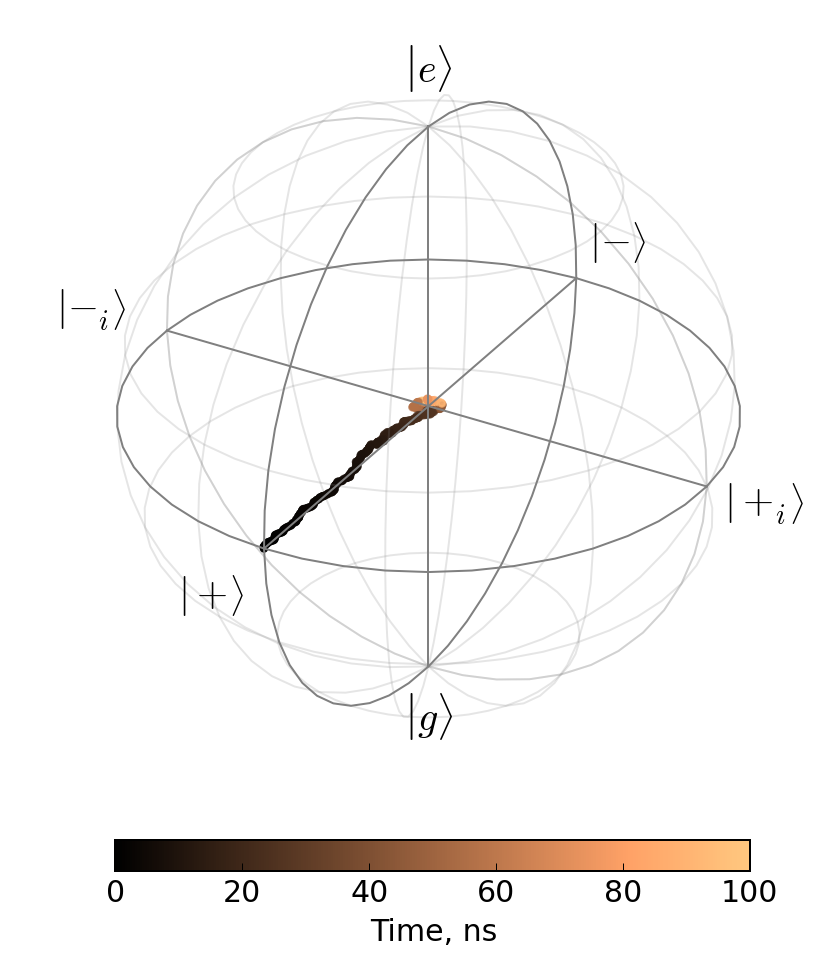
\includegraphics[width=0.9\textwidth]{cdeph_bloch_rf_avg}
\caption{Averaged dynamics in the rotating frame.}
\end{subfigure}

\begin{subfigure}[t]{0.45\textwidth}
\centering
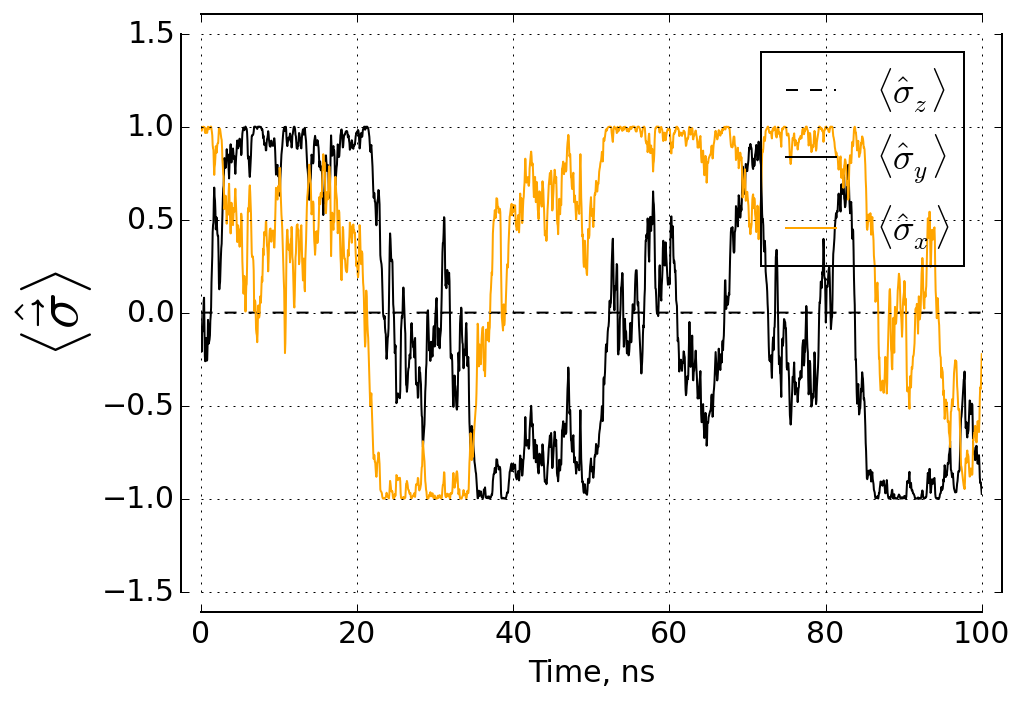
\includegraphics[width=0.9\textwidth]{cdeph_xyz_rf}
\caption{Behaviour of the $xyz$ components in the rotating frame.}
\end{subfigure}
\begin{subfigure}[t]{0.45\textwidth}
\centering
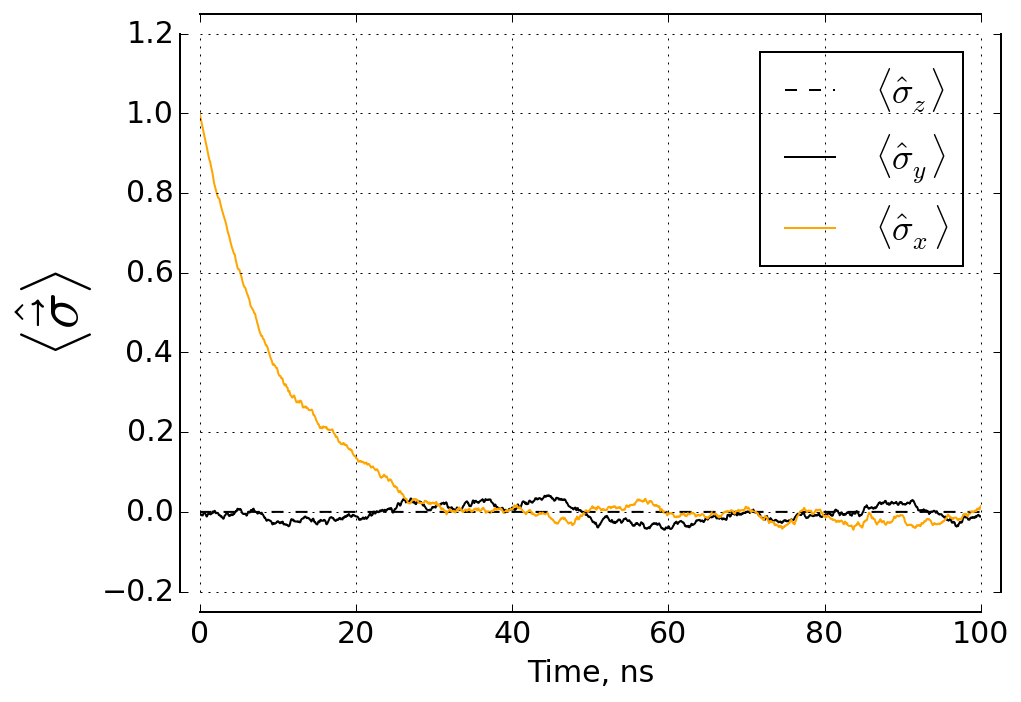
\includegraphics[width=0.9\textwidth]{cdeph_xyz_rf_avg}
\caption{Averaged behaviour of the $xyz$ components in the rotating frame.}
\end{subfigure}
\caption{Classically treated pure dephasing for white noise.}
\label{fig:cdeph}
\endgroup
\end{figure}

\begin{figure}
\begingroup
\captionsetup[subfigure]{width=0.9\textwidth}
\centering
\begin{subfigure}[t]{0.45\textwidth}
\centering
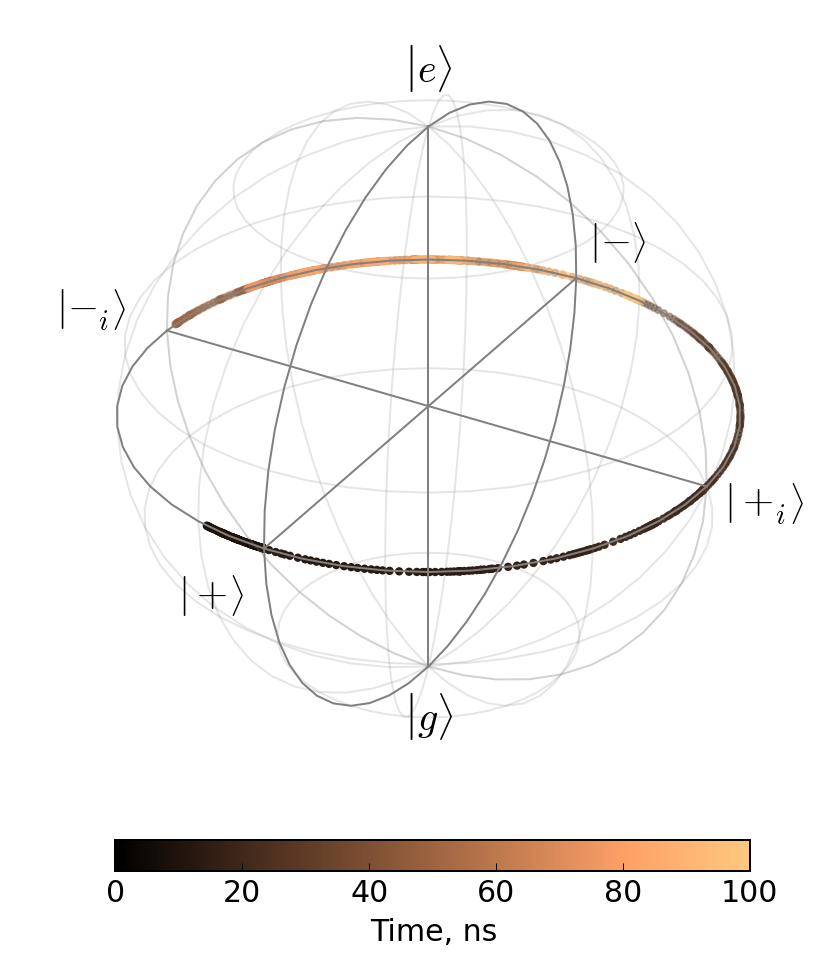
\includegraphics[width=0.9\textwidth]{cdeph_bloch_rf_pink}
\caption{1/f Gaussian noise affecting the phase in the rotating frame.}
\end{subfigure}
\begin{subfigure}[t]{0.45\textwidth}
\centering
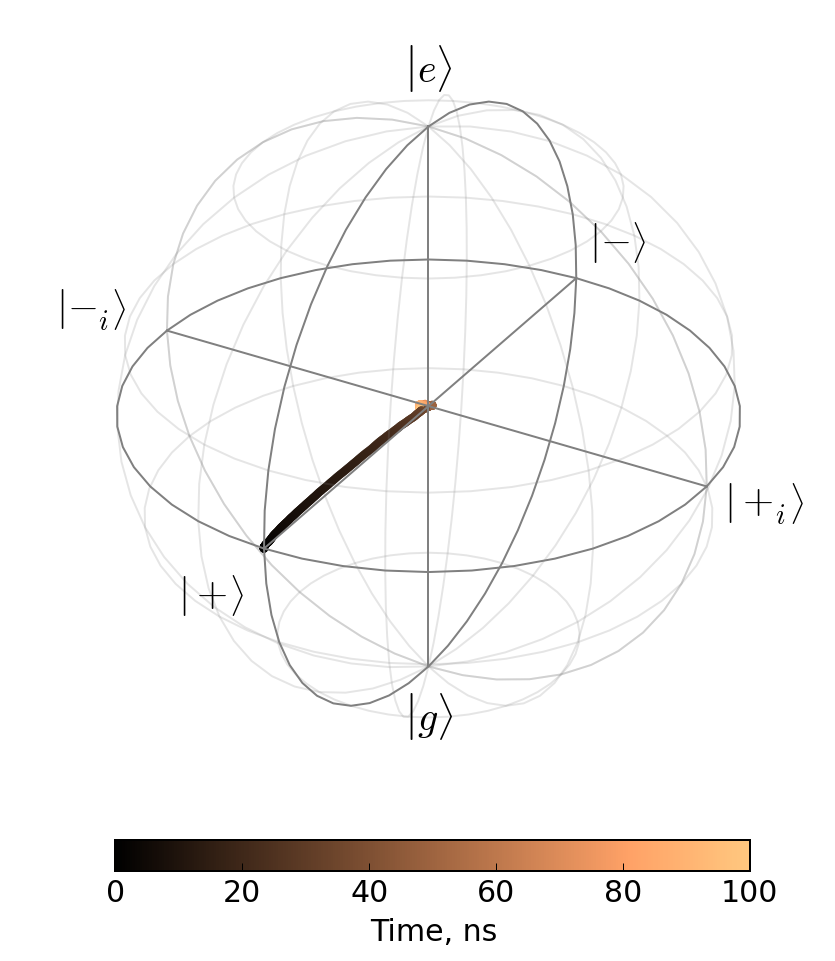
\includegraphics[width=0.9\textwidth]{cdeph_bloch_rf_avg_pink}
\caption{Averaged dynamics in the rotating frame.}
\end{subfigure}

\begin{subfigure}[t]{0.45\textwidth}
\centering
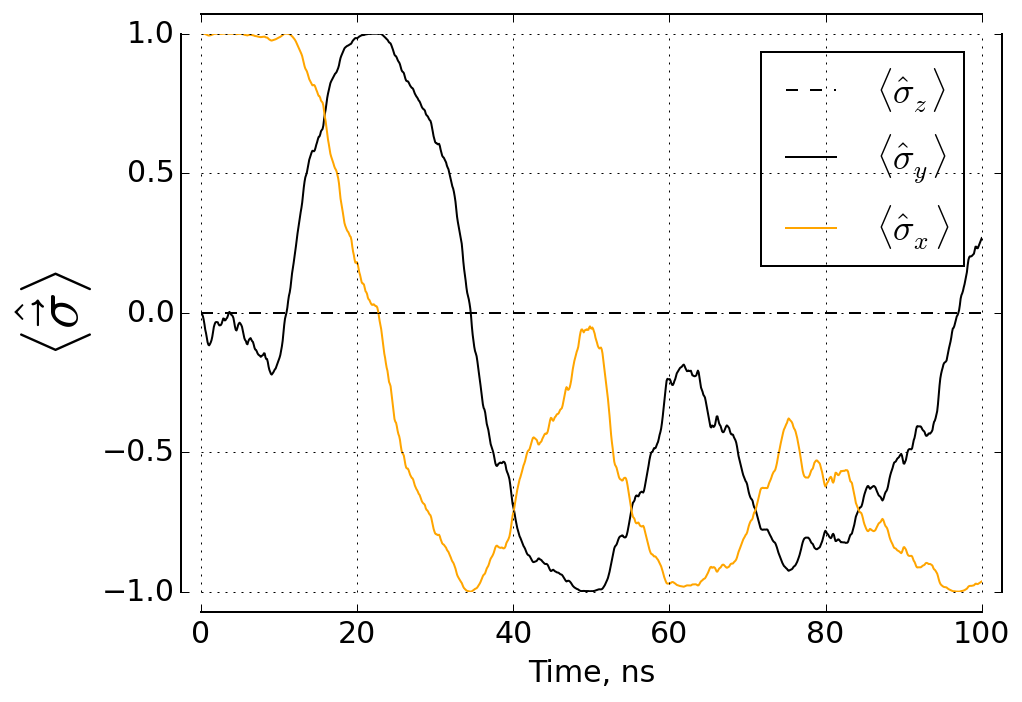
\includegraphics[width=0.9\textwidth]{cdeph_xyz_rf_pink}
\caption{Behaviour of the $xyz$ components in the rotating frame.}
\end{subfigure}
\begin{subfigure}[t]{0.45\textwidth}
\centering
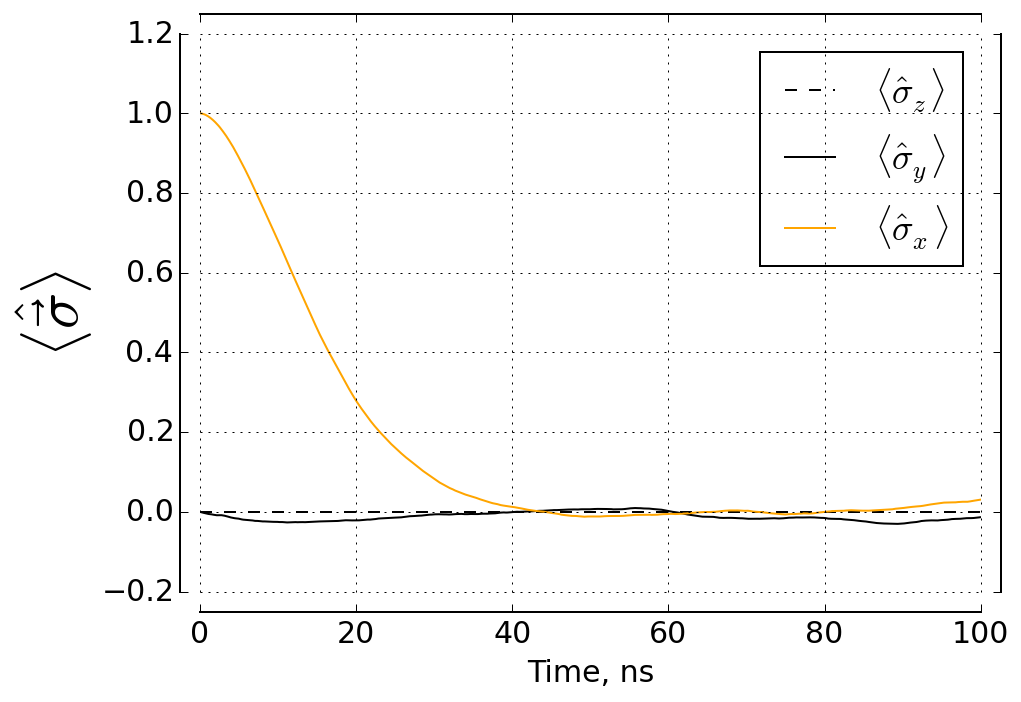
\includegraphics[width=0.9\textwidth]{cdeph_xyz_rf_avg_pink}
\caption{Averaged behaviour of the $xyz$ components in the rotating frame.}
\end{subfigure}
\caption{Classically treated pure dephasing for 1/f noise.}
\label{fig:cdeph_pink}
\endgroup
\end{figure}

\begin{figure}
\centering
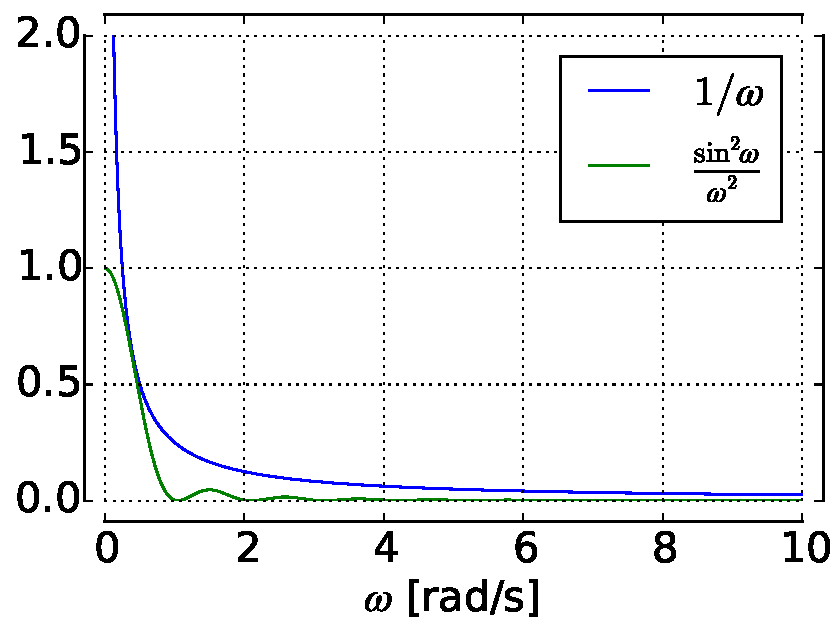
\includegraphics[width=0.4\textwidth]{ramsey_filter}\quad
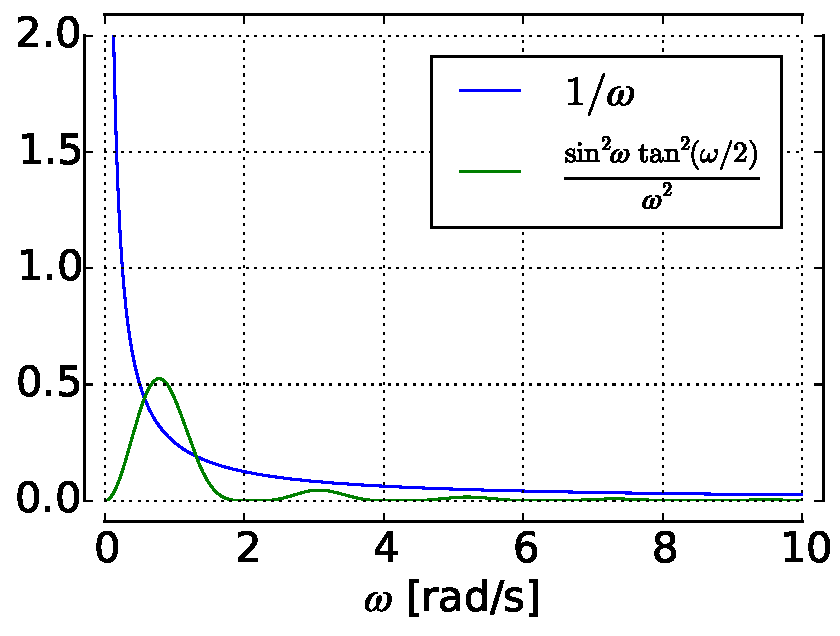
\includegraphics[width=0.4\textwidth]{hahn_filter}
\caption{Qualitative plot for noise PSD filtration at $t=10$ s.}
\end{figure}

\section{Spin-echo experiment}

The spin-echo experiment in the simplest case (Hahn echo) is a modification of a Ramsey pulse sequence with an additional $\pi_y$-pulse right in between the $\frac{\pi}{2}_x$ ones. The idea is that during the second period (after the $\pi_y$-pulse)  slow components of the noise will cancel out the phase difference they've imposed during the first period. This can be understood easily in the limit of constant noise and infinitely fast rotations. There are also more sophisticated echo sequences such as CP, CPMG and UDD\cite{Bylander2011} which use more than one $\pi_y$-pulse during the free evolution; however, for our case it is enough to regard the simplest Hahn echo.

Mathematically Hahn echo within the previous formulations acts as follows. Before the  $\pi_y$-pulse at time $t/2$ we have the same dynamics described by \eqref{eq:rho_t}. Then, instantaneously, the coherences of the density matrix are complex conjugated as a result of an infinitely fast $\pi_y$-pulse. This can be understood from the result of $\pi_y$-pulse on the Bloch sphere: $\left< \hat \sigma_x \right> = \rho + \rho^* \overset{\pi_y}{\rightarrow}  \left< \hat \sigma_x \right>,\ \left< \hat \sigma_y \right> = i(\rho - \rho^*) \overset{\pi_y}{\rightarrow} -\left< \hat \sigma_y \right>,\ \left< \hat \sigma_z \right> = N  \overset{\pi_y}{\rightarrow}  \left< \hat \sigma_z \right>$. Finally, for the changed initial condition at $t/2$ again evolution \eqref{eq:rho_t} is applied. Therefore, at the end of the period the coherence is defined as
\begin{equation*}
\rho(t) = \rho(0)\exp \left\{ - \frac{2i}{\hbar}\int_0^{t/2} f(\tau)  \diff \tau + \frac{2i}{\hbar}\int_{t/2}^{t} f(\tau)  \diff \tau \right\}.
\end{equation*}
Performing the ensemble averaging one can get
\begin{gather*}
\left<\rho(t)\right> = \rho(0)\exp \left\{ - \frac{2}{\hbar^2} \left< \left( \int_0^{t/2} f(\tau_1)  \diff \tau_1 + \int_{t/2}^{t} f(\tau_2)  \diff \tau_2 \right)\cdot \right. \right. \\
\cdot \left. \left. \left( \int_0^{t/2} f(\tau_3)  \diff \tau_3 + \int_{t/2}^{t} f(\tau_4)  \diff \tau_4 \right) \right> \right\}.
\end{gather*}
Expanding the brackets, again putting a Fourier transform of the power spectral density $S_f(\omega)$ instead of the autocorrelation functions and factoring the expression back to the initial representation it is possible to obtain\cite{Preskill} the final expression for the coherence expectation:
\begin{equation}
\left<\rho(t)\right> = \rho(0)\exp \left\{ - \frac{2}{\sqrt{2\pi} \hbar^2} \int_\mathbb{R} S_f(\omega) W^H_t (\omega) \diff\omega \right\},
\label{eq:cdeph_se}
\end{equation}
where
\begin{align*}
 W^H_t (\omega)  &= \left| - \int_0^{t/2} e^{i \omega \tau}\diff \tau + \int_{t/2}^{t} e^{i\omega\tau}  \diff \tau  \right|^2 \\
& =  \left| 1-2e^{i\omega t/2} + e^{i\omega t} \right| \\
&= \left| \frac{(1-e^{i\omega t/2})}{(1+e^{i\omega t/2})} (1+e^{i\omega t/2})(1-e^{i\omega t/2})\right|\\
& = \tan^2(\omega t/4)\frac{4 \sin^2(\omega t/2)}{\omega^2}.
\end{align*}
It's obvious from \eqref{eq:cdeph_se}  that the noise influence is now suppressed at low frequencies (compare with \eqref{eq:cdeph}) however it is enhanced at some higher frequency. This leads to inefficiency of Hahn echo and similar techniques when the noise is white and a good $T_2^*$ improvement when it's 1/f, see \autoref{fig:cdeph_both}.


\begin{figure}
\begingroup
\captionsetup[subfigure]{width=0.9\textwidth}
\centering
\begin{subfigure}[t]{0.45\textwidth}
\centering
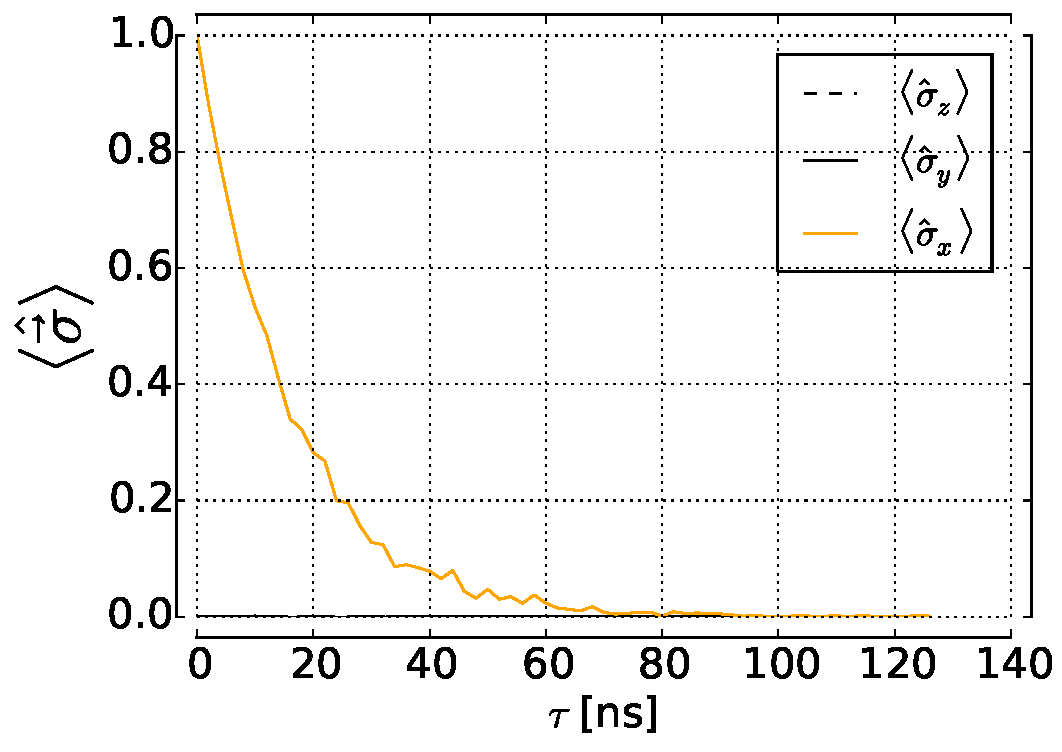
\includegraphics[width=0.9\textwidth]{deph_white}
\end{subfigure}
\begin{subfigure}[t]{0.45\textwidth}
\centering
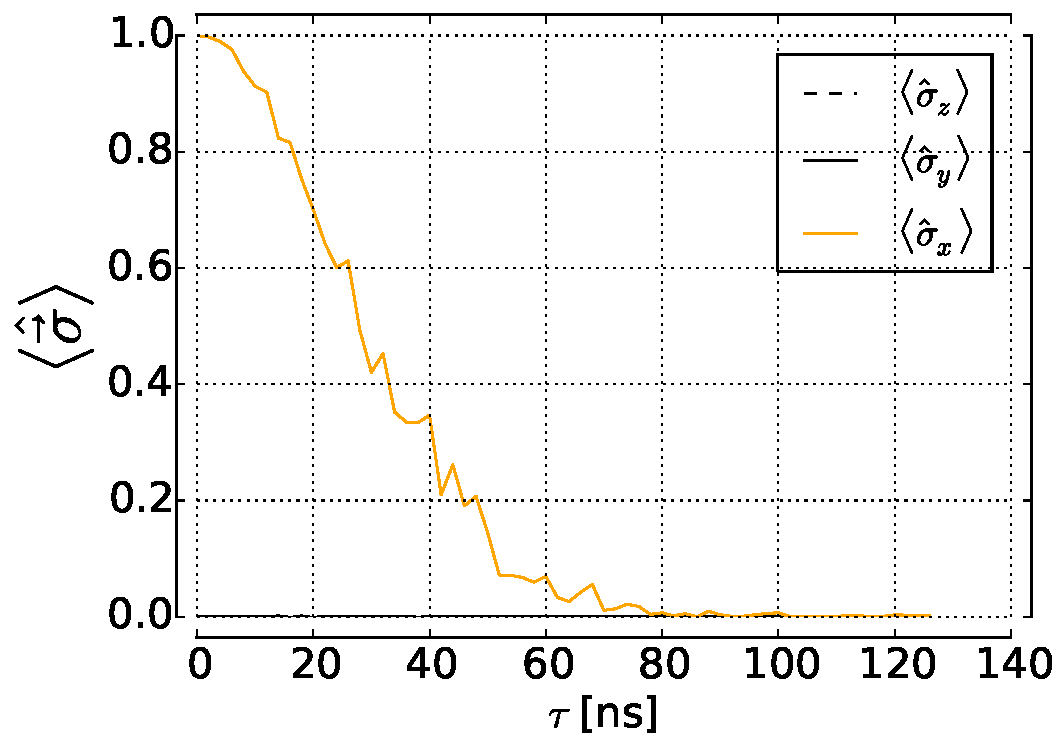
\includegraphics[width=0.9\textwidth]{deph_pink}
\end{subfigure}

\begin{subfigure}[t]{0.45\textwidth}
\centering
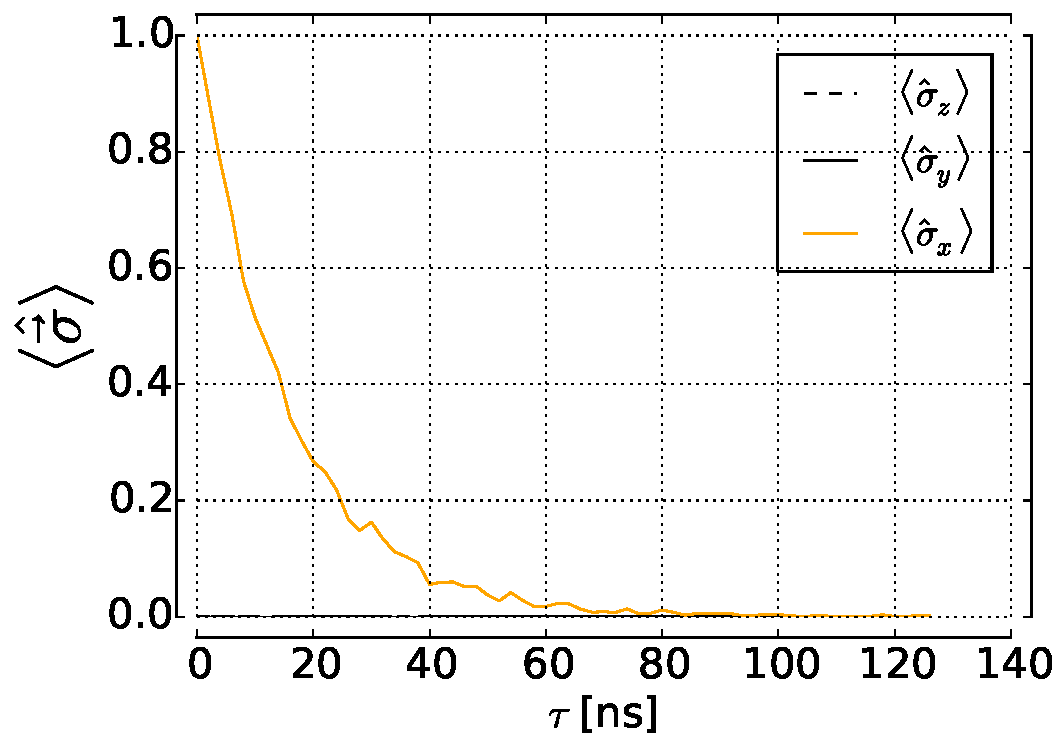
\includegraphics[width=0.9\textwidth]{deph_white_se}
\end{subfigure}
\begin{subfigure}[t]{0.45\textwidth}
\centering
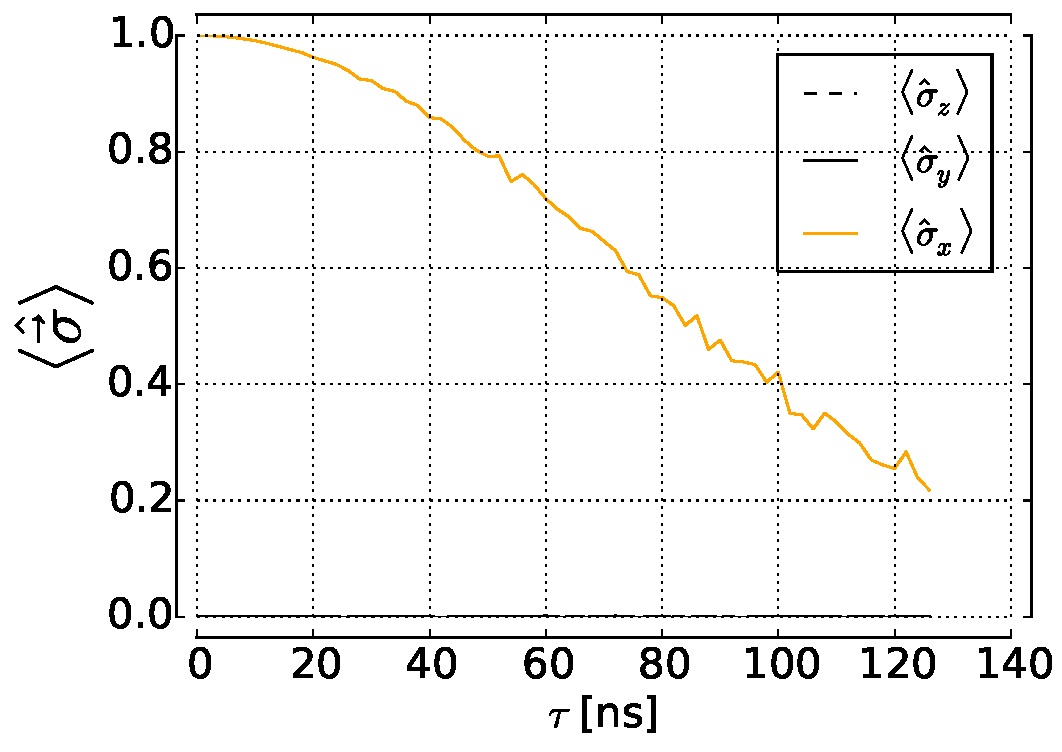
\includegraphics[width=0.9\textwidth]{deph_pink_se}
\end{subfigure}
\caption{Decoherence under white (left) and 1/f (right) noises with (bottom) and without (top) a refocusing $\pi_y$-pulse.}
\label{fig:cdeph_both}
\endgroup
\end{figure}

\section{The problem (of Markovian MEs)}

The interesting correspondence between quantum and classical derivation can be noted within the spin echo experiment. For the white noise both of the descriptions yield same results, the exponential decay of coherences with an equal rate. However the meanings of these two results are completely different. Quantum approach tells us that the density matrix will emerge even in a single experiment as a consequence of entanglement with the environment. Classical approach tells us that everything that  happens to the system in a single experiment is unitary, and if we knew the noise beforehand, we would be able to find out what state the qubit ended his evolution in at every final time $t$. Classical description only knows that the noise is white, non-correlated -- and this same idea is used in the derivation of the master equation when Markov approximation is applied.

This correspondence is lucky, but what happens if the noise \textit{is} correlated? The classical model now allows for (at least partially) reversible dynamics. In contrast, the entanglement process is completely irreversible, so the quantum model should not simply entangle the system with the environment for the correlated bath.

At this point it is safe to say that density matrix really exists (that means it is not just a way to describe statistical distribution of states, but is the only approach to describe an open quantum system), but the quantum model of decoherence for the correlated noise should go beyond the Markovian master equations to keep up with experiments and naive (but still correct!) classical description.\cite{Zurek2003}

\begin{figure}
\begingroup
\captionsetup[subfigure]{width=0.9\textwidth}
\centering
\begin{subfigure}[t]{0.45\textwidth}
\centering
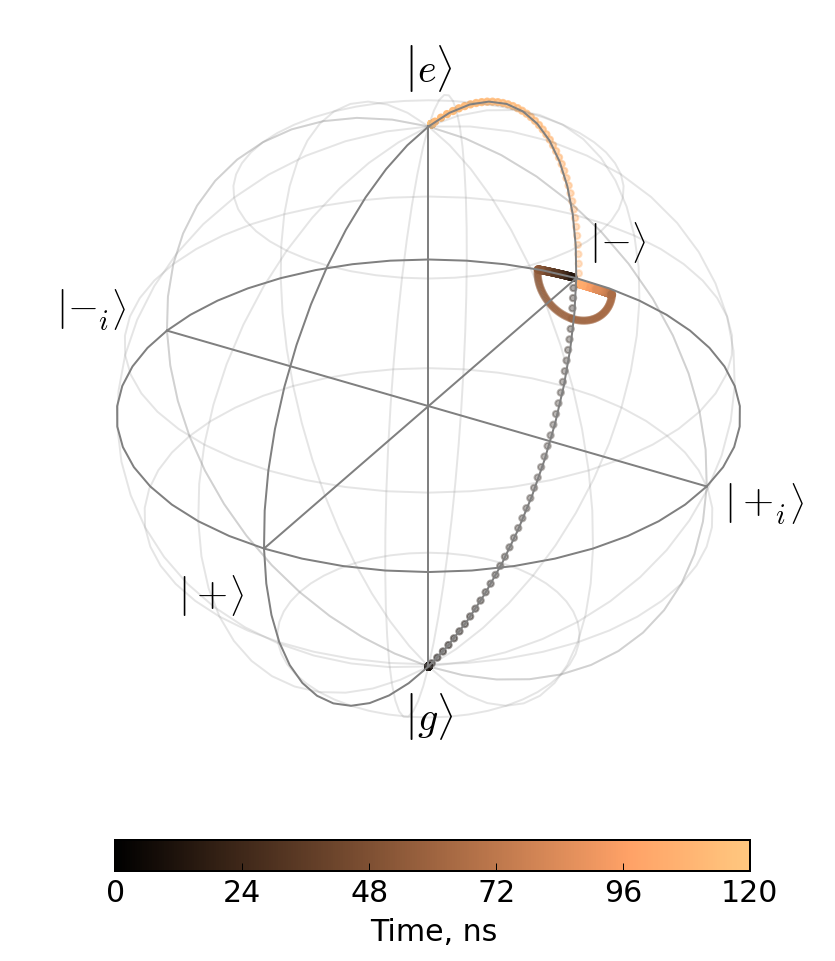
\includegraphics[width=0.9\textwidth]{cse_bloch_rf}
\caption{Schrödinger equation solution with driving and classical dephasing caused by the single $S(0)$ spectral component of the noise.}
\end{subfigure}
\begin{subfigure}[t]{0.45\textwidth}
\centering
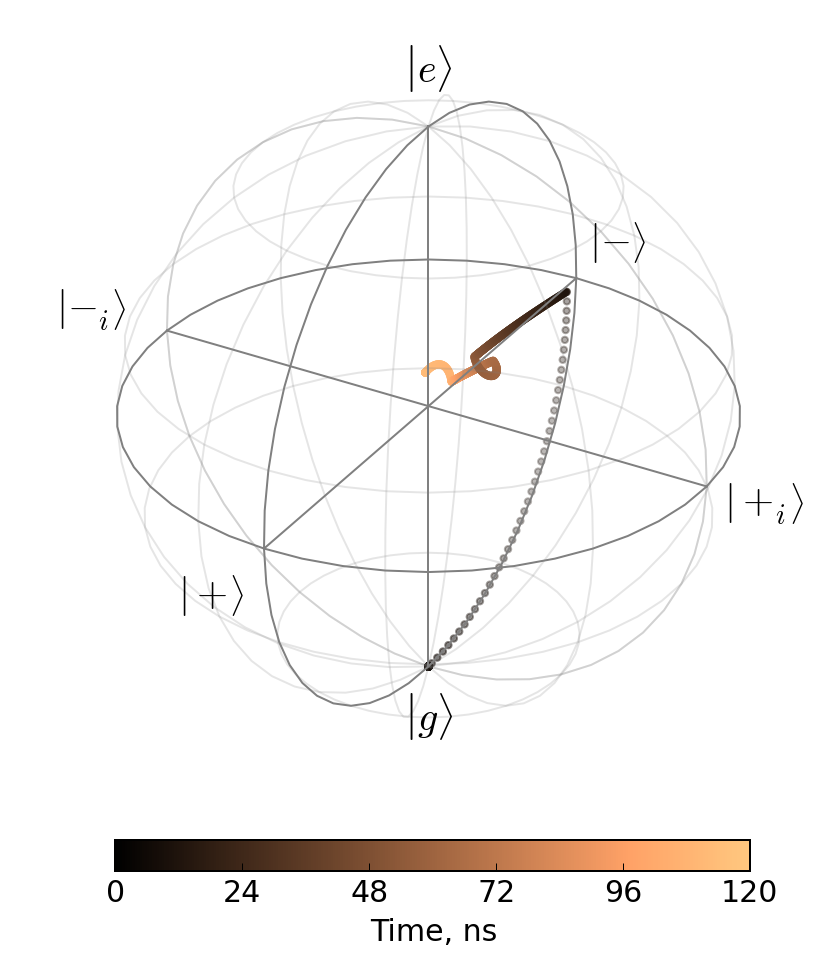
\includegraphics[width=0.9\textwidth]{qse_bloch_rf}
\caption{Master equation solution with driving and quantum dephasing.}
\end{subfigure}

\begin{subfigure}[t]{0.45\textwidth}
\centering
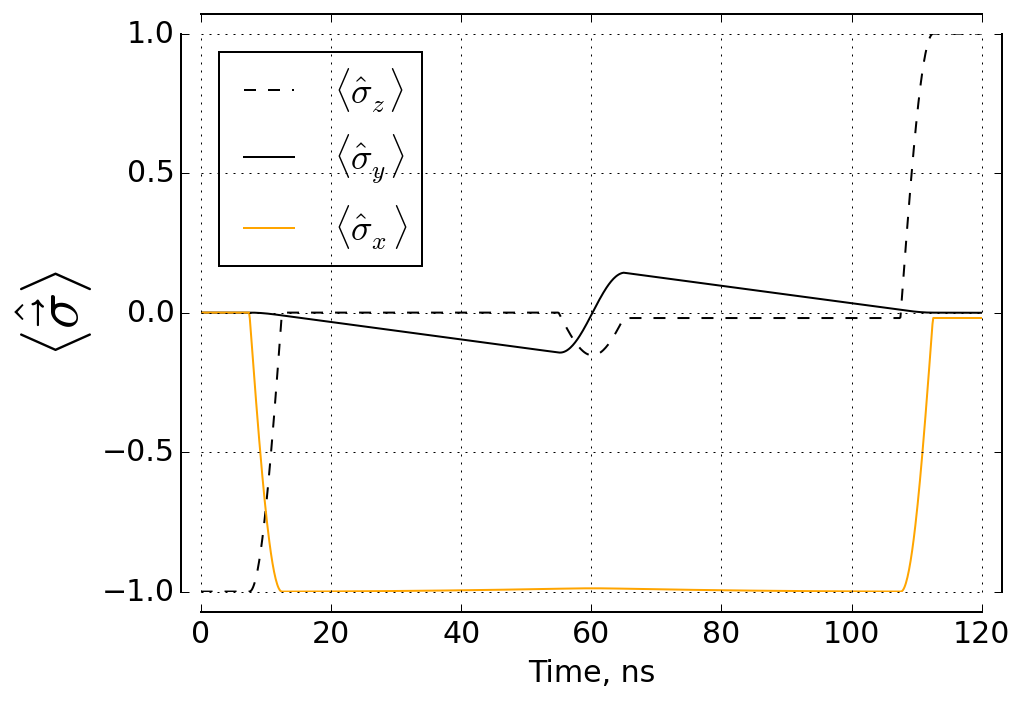
\includegraphics[width=0.99\textwidth]{cse_xyz_rf}
\caption{Same in $xyz$. Dephasing is linear in time and reversible for this case.}
\end{subfigure}
\begin{subfigure}[t]{0.45\textwidth}
\centering
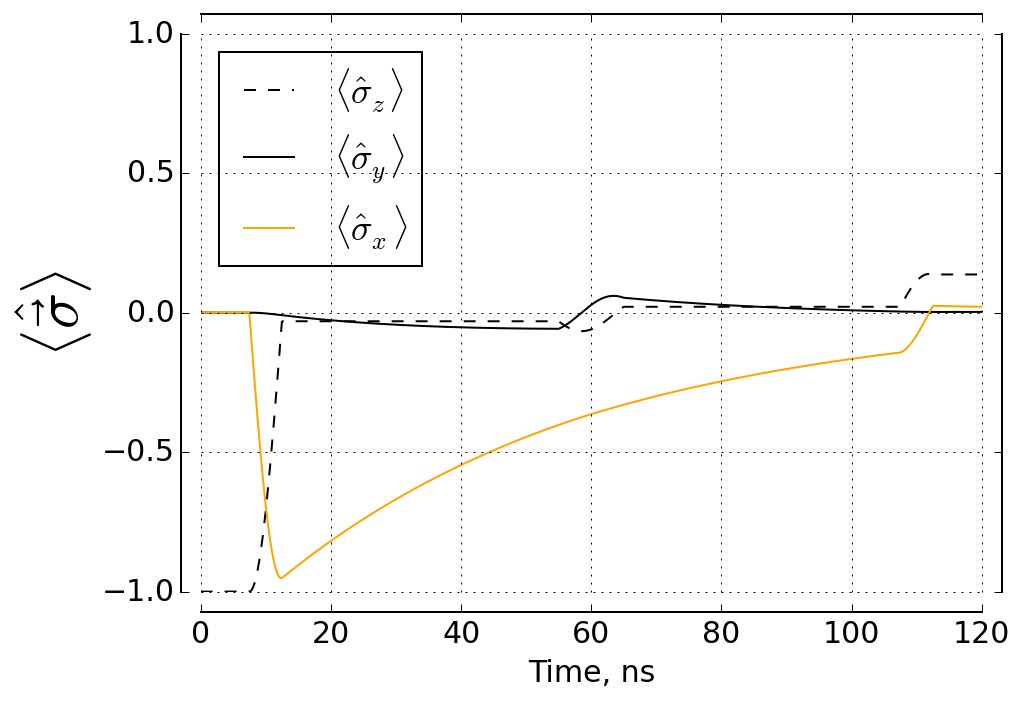
\includegraphics[width=0.99\textwidth]{qse_xyz_rf}
\caption{Same in $xyz$. Dephasing destroys the coherence and is irreversible.}
\end{subfigure}
\caption{Classical versus quantum spin-echo experiment modelling. Spin-echo can't cope with quantum noise.}
\label{fig:se}
\endgroup

\end{figure}